%        File: FireflySpec_1p0.tex
%     Created: Thu Jan 17 01:00 PM 2019 E
%
\documentclass[letterpaper,11pt]{article}
\usepackage[leqno]{amsmath}
\usepackage{mathptmx,courier}
\usepackage[scaled]{helvet}
\usepackage[inter-unit-product=\ensuremath{{}\cdot{}},per-mode=symbol,separate-uncertainty,binary-units]{siunitx}
\usepackage[letterpaper,lmargin=0.75in,rmargin=0.75in,tmargin=0.75in,bmargin=0.75in]{geometry}
\usepackage{paralist}
\usepackage{supertabular}
\usepackage[pdftex]{graphicx}
\usepackage[hyperfigures=false,bookmarks=false,pdftex,colorlinks,linkcolor=black,urlcolor=blue]{hyperref}
\usepackage[cachedir=/home/kjh016/tmp/mintedcache]{minted}

\graphicspath{{graphics/}}

\ifpdf\pdfinfo{
  /Title (Firefly Simulator Specification) %FIXME
  /Author (Bucknell University) %FIXME
/Keywords () }
\fi

% load hyperref package first!!
\usepackage{fancyhdr,pageslts}
\pagestyle{fancy}
\fancyhf{}
\fancyhead[L]{Firefly Simulator Specification}
\fancyfoot[C]{Page \thepage\ of \pageref*{LastPage}}
\usepackage[iso]{datetime}
\fancyfoot[L]{Revised \today}
\pagenumbering{arabic}
\renewcommand\headrulewidth{0pt}

\begin{document}
\section{Overview}

This document provides specifications for a \textit{firefly simulator}. This
device is intended to simulate the light displays of common fireflies, such
as \textit{Photinus pyralis}. The \textit{firefly simulator} will provide means
to control the brightness, duration, and other relevant parameters of the
simulated light display. Light-emitting diodes (LEDs) will be used as the light
source, and the color of the display can be altered by connecting different
LED types to the simulator.

The \textit{firefly simulator} can be configured via commands issued to it
from a host computer, as shown in Fig.\ \ref{fig:blockdiagram}. The physical
link between the host computer and the \textit{firefly simulator} is an
asynchronous serial communications interface, which can be accomplished with a
common and inexpensive USB adapter. The \textit{firefly simulator} also can
return status information to the host computer via the same interface.

Once configured, the \textit{firefly simulator} can be used in a stand-alone
mode, without requiring a connection to a host computer. Pushbuttons on the
\textit{firefly simulator} can be used to activate light displays that were
previously configured. When in the stand-alone mode, the simulator can be
powered by a USB powerbank.

\begin{figure}[h]
  \begin{center}
    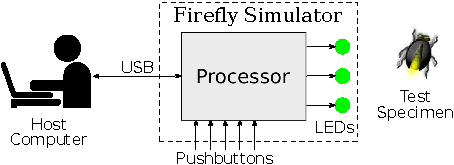
\includegraphics[scale=1.5]{Flashes_BlockDiagram}
  \end{center}
  \vspace{-18pt}
  \caption{Firefly Simulator Block Diagram}
  \label{fig:blockdiagram}
\end{figure}

This document describes the minimum required functionality of the
\textit{firefly simulator}. Possible future enhancements to the simulator
include:
\begin{compactitem}
  \item The ability to sense the behavior of a test specimen and use that
    behavior to modify the parameters of a light display.
  \item The ability to record information about simulator activity on
    non-volatile memory, such as a removable Secure Digital (SD) memory card.
  \item The addition of a real-time clock (RTC) to the \textit{firefly
    simulator} so that timestamps can be added to response messages from the 
    simulator to the host computer.
\end{compactitem}

\section{References}

\textit{IEEE Standard for Transitions, Pulses, and Related Waveforms},
  IEEE Standard 181, 2011.

\section{Definitions}

\begin{figure}[h]
  \begin{center}
    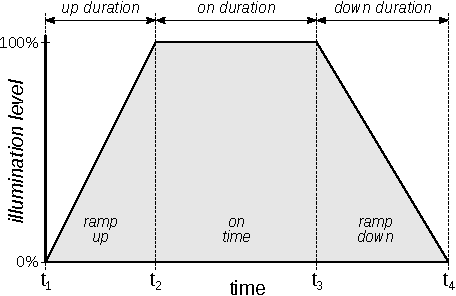
\includegraphics{Flashes_BlinkPulse}
  \end{center}
  \vspace{-18pt}
  \caption{\textit{blink} waveform}
  \label{fig:blinkpulse}
\end{figure}

\setlength\extrarowheight{4pt}
\begin{supertabular}{p{1.5in}p{5in}}
ASCII &
    The American Standard Code for Information Interchange. The letters in
    the English alphabet, the decimal digits, and common punctuation marks are
    assigned a unique 7-bit binary code.\\
blink &
    The process of bringing the \textit{illumination level} of an \textit{LED}
    from 0\% to 100\% then back to 0\% illumination. A \textit{blink} consists of
    a \textit{ramp up}, followed by an \textit{on time}, followed by a
    \textit{ramp down}. A \textit{blink} begins at $t_1$ and ends at $t_4$,
    as shown in Fig.\ \ref{fig:blinkpulse}. The interval from $t_1$ to $t_2$
    is the \textit{ramp up}. The interval from $t_2$ to $t_3$ is the \textit{on
    time}.  The interval from $t_3$ to $t_4$ is the \textit{ramp down}. \\
channel &
    The \textit{channel} of an \textit{LED} is an integer that specifies
    which physical output connector of the firefly simulator is connected
    to the physical LED. The value of \textit{channel} is an integer and
    shall not be less than 1 and not greater than \textit{max channel}.\\
        &
    Note that the \textit{channel} is not the pin number of any particular
    microcontroller. An implementation of the firefly simulator must perform
    the appropriate mapping of an \textit{LED}'s \textit{channel} to an
    appropriate physical pin on the output device.\\
down duration & 
    The length of the \textit{ramp down} interval. The \textit{down duration}
    is equal to $t_4 - t_3$, as shown in Fig.\ \ref{fig:blinkpulse}. The
    \textit{down duration} shall be a non-negative integer value with units
    of milliseconds. The value of \textit{down duration} shall not be less
    than 0 or greater than 32\,767.\\
%duty factor &  For a periodic rectangular pulse that has only two possible
%    voltage levels, the \textit{duty factor} is the ratio of the duration of
%    the pulse at its higher voltage divided by the period of the waveform.
%
%    \[ 0.0 \le d_f \le 1.0 \quad \mathrm{ or } \quad 0\% \le d_f \le 100\%\]
illumination level &
    The brightness of an \textit{LED} at any given point in time, as a
    percentage of that \textit{LED}'s \textit{max brightness}. The
    \textit{illumination level} and \textit{max brightness} values
    indirectly translate to the average current passing through the physical
    LED.\\
    &
    At any given point in time, the average current for an LED is
\[ I_{AVG} = \frac{illumination\,level}{100} \times \frac{max\,brightness}{100}
\times I_{max}\]\\
message &  A sequence of \textit{message fields}, separated by the
    ASCII comma character (decimal 44) and terminated by either the ASCII Line
    Feed (decimal 10), the ASCII Carriage Return (decimal 13), or both the Line
    Feed and the Carriage Return. There shall not be a comma before the first
    field in a message nor after the last field.\\
message field &  A sequence of one or more ASCII characters from the
    set of uppercase letters (\texttt{A} through \texttt{Z}) and decimal digits
    (\texttt{0} through \texttt{9}). A message field shall not include
    any characters or values other than the uppercase letters and decimal
    digits.\\
max brightness & 
    The maximum duty factor of the \textit{pulse-width modulation} signal that
    controls the \textit{illumination level} of an \textit{LED}. The
    \textit{max brightness} is a characteristic of an \textit{LED}. The
    value of \textit{max brightness} is an integer and shall be not less
    than 1 and not greater than 100.\\
max channel & 
    The number of physical \textit{LED} \textit{channels} available on a
    particular implementation of a \textit{firefly simulator}.
    The value of \textit{max channel} shall not be less than 1 or greater
    than 127 for any implementation of a \textit{firefly simulator}.\\
max blink & 
    The number of unique \textit{blink} configurations available on a
    particular implementation of a \textit{firefly simulator}.
    The value of \textit{max blink} shall not be less than 1 or greater
    than 127 for any implementation of a \textit{firefly simulator}.\\
max pattern & 
    The number of unique \textit{pattern} configurations available on a
    particular implementation of a \textit{firefly simulator}.
    The value of \textit{max pattern} shall not be less than 1 or greater
    than 127 for any implementation of a \textit{firefly simulator}.\\
on duration &
    The length of the \textit{on time} interval. The \textit{on duration} is
    equal to $t_3 - t_2$, as shown in Fig.\ \ref{fig:blinkpulse}. The value
    of \textit{on duration} shall be a positive, non-zero integer with units
    of milliseconds. The value of \textit{on duration} shall not be less than 1
    or greater than 32\,767.\\
on time &
    The period of time during a \textit{blink} when the \textit{LED} is
    constantly at an illumination level of 100\%.\\
pattern &
    A sequence of up to four \textit{blinks} with user-specified delays before
    each \textit{blink}, as shown in Fig.\ \ref{fig:patterntimeline}.\\
%pulse-width modulation & 
ramp down &
    The process of linearly decreasing the \textit{illumination level} of an
    \textit{LED} from 100\% to 0\%.\\
ramp up &
    The process of linearly increasing the \textit{illumination level} of an
    \textit{LED} from 0\% to 100\%.\\
up duration &
    The length of the \textit{ramp up} interval. The \textit{up duration}
    is equal to $t_2 - t_1$, as shown in Fig.\ \ref{fig:blinkpulse}. The
    value of \textit{up duration} shall be a non-negative integer with units
    of milliseconds. The value of \textit{up duration} shall not be less than
    0 or greater than 32\,767.\\
\end{supertabular}

\begin{figure}[t]
  \begin{center}
    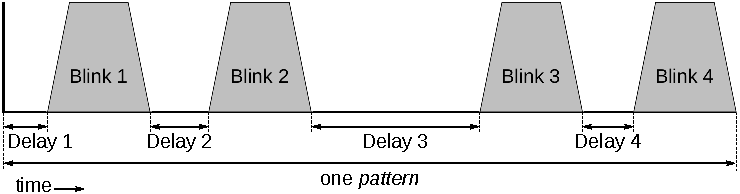
\includegraphics{Flashes_PatternTimeline}
  \end{center}
  \vspace{-18pt}
  \caption{\textit{pattern} timeline (without a \textit{wait event})}
  \label{fig:patterntimeline}
\end{figure}

\section{Resolution and Accuracy}

\subsection{Brightness}

The \textit{firefly simulator} does not directly control the brightness of a
physical LED. Instead, the simulator controls the average current provided to
the LED. The simulator's configuration messages allow the actual average
current ($I_{AVG}$) of an LED to be specified with a resolution of $\pm 1$\% of
the maximum available current ($I_{MAX}$). The maximum available current, and
the precision which with the current can be specified, will be
determined by the circuitry associated with a given physical LED and need not be
the same for all LEDs.

\subsection{Time}

Values that represent time shall have units of milliseconds and a resolution
of \SI{1}{\milli\second}. The accuracy of all pulse durations and time delays
generated by the \textit{firefly simulator} shall have a maximum error of
\SI{\pm 10}{\milli\second}.

\newpage
\section{Configuration Messages}

The firefly simulator is configured via a serial communications interface to
a host computer. The host computer can set the values of all parameters for
\textit{LEDs}, \textit{blinks}, and \textit{patterns}. A unique configuration
message format is specified for configuring an \textit{LED}, configuring a
\textit{blink}, or configuring a \textit{pattern}.

\subsection{\textit{capacity query/capacity response messages}}

The \textit{capacity query message} can be used by the host computer to
determine the capabilities of a \textit{firefly simulator}.

\begin{table}[H]
  \caption{Definition of \textit{capacity query message}}
  \centering
  \setlength\extrarowheight{2pt}
  \begin{tabular}[h]{|p{0.5in}|p{1.00in}|p{2.25in}|p{2.25in}|} \hline
    Field Number & Field Name & Description & Format \\ \hline
    1            & Header
    & Unique first character for an \textit{capacity query message}
    & This field shall be the uppercase letter `\texttt{C}'.
    \\ \hline
  \end{tabular}
  \label{tab:CapacityQuery}
\end{table}

The \textit{firefly simulator} will respond to the \textit{capacity query
message} by sending a \textit{capacity response message} to the host computer.

\begin{table}[H]
  \caption{Definition of \textit{capacity response message}}
  \centering
  \setlength\extrarowheight{2pt}
  \begin{tabular}[h]{|p{0.5in}|p{1.00in}|p{2.25in}|p{2.25in}|} \hline
    Field Number & Field Name & Description & Format \\ \hline
    1            & \textit{max channel}
    & The number of physical LEDs available
    & This field shall contain a decimal integer from 1 to 127.
    \\ \hline
    2            & \textit{max blink}
    & The number of available \textit{blink} definitions
    & This field shall contain a decimal integer from 1 to 127.
    \\ \hline
    3            & \textit{max pattern}
    & The number of available \textit{pattern} definitions
    & This field shall contain a decimal integer from 1 to 127.
    \\ \hline
  \end{tabular}
  \label{tab:CapacityResponse}
\end{table}

\subsection{\textit{LED configuration message}}

An \textit{LED configuration message} is sent from the host computer to the
firefly simulator. Every \textit{LED configuration message} shall contain
three \textit{message fields}, as shown in Table \ref{tab:LEDconfig}.

\begin{table}[H]
  \caption{Definition of \textit{LED configuration message}}
  \centering
  \setlength\extrarowheight{2pt}
  \begin{tabular}[h]{|p{0.5in}|p{1.00in}|p{2.25in}|p{2.25in}|} \hline
    Field Number & Field Name & Description & Format \\ \hline
    1            & Header
    & Unique first character for an \textit{LED configuration message}
    & This field shall be the uppercase letter `\texttt{L}'.
    \\ \hline
    2            & LED \textit{channel}
    & A unique identifier for each physical LED
    & This field shall contain a decimal integer from 1 to \textit{max channel}.
    \\ \hline
    3            & \textit{max brightness}
    & The maximum brightness level for the LED
    & This field shall contain a decimal integer from 1 to 100.
    \\ \hline
  \end{tabular}
  \label{tab:LEDconfig}
\end{table}

\subsection{\textit{blink configuration message}}

An \textit{blink configuration message} is sent from the host computer to the
firefly simulator. This message provides the parameters for a single
\textit{blink} of an \textit{LED}, as shown in Table \ref{tab:BlinkConfig}.

\begin{table}[H]
\centering
\caption{Definition of a \textit{blink configuration message}}
\label{tab:BlinkConfig}
\setlength\extrarowheight{2pt}
\begin{tabular}[h]{|p{0.5in}|p{1.00in}|p{2.25in}|p{2.25in}|} \hline
Field Number & Field Name & Description & Format \\ \hline
1            & Header
             & Unique first character for a \textit{blink configuration message}
             & This field shall be the uppercase letter `\texttt{B}'.
             \\ \hline
2            & \textit{blink} number
             & A unique identifier for each \textit{blink} definition
             & This field shall contain a decimal integer from 1 to
             \textit{max blink}.
             \\ \hline
3            & LED number
             & Identifier for the \textit{LED} to be illuminated in this
             \textit{blink}
             & This field shall contain a decimal integer from 1 to
             \textit{max channel}.
             \\ \hline
4            & \textit{up duration}
             & The duration of the \textit{ramp up} in milliseconds
             & This field shall contain a decimal integer from 0 to 32\,767.
             \\ \hline
5            & \textit{on duration}
             & The duration of the \textit{on time} in milliseconds
             & This field shall contain a decimal integer from 1 to 32\,767.
             \\ \hline
6            & \textit{down duration}
             & The duration of the \textit{ramp down} in milliseconds
             & This field shall contain a decimal integer from 0 to 32\,767.
             \\ \hline
\end{tabular}
\end{table}

\subsection{\textit{pattern configuration message}}

An \textit{pattern configuration message} is sent from the host computer to the
firefly simulator. This message provides the parameters for a single
\textit{pattern} of one or more \textit{blinks}, as shown in Table
\ref{tab:PatternConfig}. Note that the same \textit{blink} may be repeated
within a pattern or up to four different \textit{blinks} may be combined.

\begin{table}[H]
\centering
\caption{Definition of a \textit{pattern configuration message}}
\label{tab:PatternConfig}
\setlength\extrarowheight{2pt}
\begin{tabular}[h]{|p{0.5in}|p{1.00in}|p{2.25in}|p{2.25in}|} \hline
Field Number & Field Name & Description & Format \\ \hline
1            & Header
             & Unique first character for a \textit{pattern configuration
             message}
             & This field shall be the uppercase letter `\texttt{P}'.
             \\ \hline
2            & \textit{pattern} number
             & A unique identifier for each \textit{pattern} definition
             & This field shall be a decimal integer from 1 to \textit{max
             pattern}.
             \\ \hline
3            & Delay 1
             & The duration of the delay from the beginning of the pattern
               to the first \textit{blink}, in milliseconds
             & This field shall contain a decimal integer from 0 to 32767.
             \\ \hline
4            & Blink 1
             & The identifier of the first \textit{blink} in the pattern
             & This field shall contain a decimal integer from 0 to
             \textit{max blink}. A value of 0 causes this blink to be omitted
             from the pattern.
             \\ \hline
5            & Delay 2
             & The duration of the delay from the end of the first
               \textit{blink} to the beginning of the second \textit{blink},
               in milliseconds
             & This field shall contain a decimal integer from 0 to 32767.
             \\ \hline
6            & Blink 2
             & The identifier of the second \textit{blink} in the pattern
             & This field shall contain a decimal integer from 0 to
             \textit{max blink}. A value of 0 causes this blink to be omitted
             from the pattern.
             \\ \hline
7            & Wait 1
             & The identifier of a \textit{wait event}
             & This field shall be a single decimal digit from `0' to `9'. A
               value of `0' indicates that there is no \textit{wait event}.
             \\ \hline
8            & Delay 3
             & The duration of the delay inserted before the beginning of the
               third \textit{blink}, in milliseconds
             & This field shall contain a decimal integer from 0 to 32767.
             \\ \hline
9            & Blink 3
             & The identifier of the third \textit{blink} in the pattern
             & This field shall contain a decimal integer from 0 to
             \textit{max blink}. A value of 0 causes this blink to be omitted
             from the pattern.
             \\ \hline
10           & Delay 3
             & The duration of the delay from the end of the third
               \textit{blink} to the beginning of the fourth \textit{blink},
               in milliseconds
             & This field shall contain a decimal integer from 0 to 32767.
             \\ \hline
11           & Blink 4
             & The identifier of the fourth \textit{blink} in the pattern
             & This field shall contain a decimal integer from 0 to
             \textit{max blink}. A value of 0 causes this blink to be omitted
             from the pattern.
             \\ \hline
\end{tabular}
\end{table}

\newpage
\section{Command Messages}

The host computer can command the \textit{firefly simulator} to turn on an
\textit{LED} at a specified \textit{illumination level}, execute a specific
\textit{blink}, execute a specific \textit{pattern}, or execute all available
\textit{patterns} in a pseudorandom order.

\subsection{\textit{Execute LED message}}

An \textit{Execute LED message} is sent from the host computer to the
firefly simulator. This message can be used to turn an LED on or off for
testing or calibration purposes. Every \textit{Execute LED message} shall
contain three \textit{message fields}, as shown in Table \ref{tab:ExecuteLED}.

\begin{table}[H]
  \caption{Definition of \textit{Execute LED message}}
  \centering
  \setlength\extrarowheight{2pt}
  \begin{tabular}[h]{|p{0.5in}|p{1.00in}|p{2.25in}|p{2.25in}|} \hline
    Field Number & Field Name & Description & Format \\ \hline
    1            & Header
                 & Unique first two characters for an \textit{Execute LED
                 message}
                 & This field shall be the uppercase letters `\texttt{XL}'.
                 \\ \hline
    2            & LED \textit{channel}
                 & A unique identifier for a physical LED
                 & This field shall contain a decimal integer from 1 to
                 \textit{max channel}.
                 \\ \hline
    3            & \textit{illumination level}
                 & Sets a constant value for the \textit{illumination level}
                 of the \textit{LED}
                 & This field shall contain a decimal integer from 0 to 100.
                 A value of 100 causes the \textit{illumination level} of the
                 LED to be set at a constant value of 100\% (of the
                 \textit{LED}'s \textit{max brightness} level). A `0' shall
                 cause the \textit{illumination level} of the LED to be set at
                 0\% (completely dark).
                 \\ \hline
  \end{tabular}
  \label{tab:ExecuteLED}
\end{table}

\subsection{\textit{Execute blink message}}

An \textit{Execute blink message} is sent from the host computer to the
firefly simulator. This message can be used to cause the firefly simulator to
repeatedly execute a specific \textit{blink} sequence. Every \textit{Execute
blink message} shall contain three \textit{message fields}, as shown in Table
\ref{tab:ExecuteBlink}.

This command can be terminated before the simulator reaches the specified
repeat count by \textbf{TBD}.

\begin{table}[H]
  \caption{Definition of \textit{Execute blink message}}
  \centering
  \setlength\extrarowheight{2pt}
  \begin{tabular}[h]{|p{0.5in}|p{1.00in}|p{2.25in}|p{2.25in}|} \hline
    Field Number & Field Name & Description & Format \\ \hline
    1            & Header
                 & Unique first two characters for an \textit{Execute blink
                 message}
                 & This field shall be the uppercase letters `\texttt{XB}'.
                 \\ \hline
    2            & \textit{blink} number
                 & A unique identifier for a \textit{blink}
                 & This field shall contain a decimal integer from 1 to
                 \textit{max blink}.
                 \\ \hline
    3            & Repeat
                 & A positive, non-zero integer value specifying the number
                 of times that the \textit{blink} should be repeated. 
                 & This field shall a decimal integer from 1 to 32\,767.
    \\ \hline
  \end{tabular}
  \label{tab:ExecuteBlink}
\end{table}

\subsection{\textit{Execute pattern message}}

An \textit{Execute pattern message} is sent from the host computer to the
firefly simulator. This message can be used to cause the firefly simulator to
repeatedly execute a specific \textit{pattern}. Every \textit{Execute pattern
message} shall contain three \textit{message fields}, as shown in Table
\ref{tab:ExecutePattern}.

This command can be terminated before the simulator reaches the specified
repeat count by \textbf{TBD}.

\begin{table}[H]
  \caption{Definition of \textit{Execute pattern message}}
  \centering
  \setlength\extrarowheight{2pt}
  \begin{tabular}[h]{|p{0.5in}|p{1.00in}|p{2.25in}|p{2.25in}|} \hline
    Field Number & Field Name & Description & Format \\ \hline
    1            & Header
                 & Unique first two characters for an \textit{Execute pattern
                 message}
                 & This field shall be the uppercase letters `\texttt{XP}'.
                 \\ \hline
    2            & \textit{pattern} number
                 & A unique identifier for a \textit{pattern}
                 & This field shall contain a decimal integer from 1 to
                 \textit{max pattern}.
                 \\ \hline
    3            & Repeat
                 & A positive, non-zero integer value specifying the number of
                 times that the \textit{pattern} should be repeated. 
                 & This field shall a decimal integer from 1 to 32\,767.
                 \\ \hline
  \end{tabular}
  \label{tab:ExecutePattern}
\end{table}

\subsection{\textit{Execute random pattern message}}

An \textit{Execute random pattern message} is sent from the host computer to the
\textit{firefly simulator}. This message can be used to cause the simulator to
pseudo-randomly select and execute patterns from the set of all configured
patterns. The simulator will continuously execute patterns until \textbf{TBD}.

\begin{table}[H]
  \caption{Definition of \textit{Execute random pattern message}}
  \centering
  \setlength\extrarowheight{2pt}
  \begin{tabular}[h]{|p{0.5in}|p{1.00in}|p{2.25in}|p{2.25in}|} \hline
    Field Number & Field Name & Description & Format \\ \hline
    1            & Header
                 & Unique first two characters for an \textit{Execute random
                 pattern message}
                 & This field shall be the uppercase letters `\texttt{XR}'.
                 \\ \hline
  \end{tabular}
  \label{tab:ExecuteRandom}
\end{table}

\end{document}
